% ==============================================================================
% thesis.tex
% Beispieldatei für tumthesis.csl
% Michael Ritter, 2012
% Lizenz: 
% This work may be distributed and/or modified under the
% conditions of the LaTeX Project Public License, either version 1.3
% of this license or (at your option) any later version.
% The latest version of this license is in
% http://www.latex-project.org/lppl.txt
% and version 1.3 or later is part of all distributions of LaTeX
% version 2005/12/01 or later.
% ==============================================================================
\documentclass[]{tumthesis}

% ------------------------------------------------------------------------------
%FixMe-Status: final (keine FixMe-Anmerkungen) oder draft (Anmerkungen sichtbar)
\fxsetup{draft}
%\fxsetup{final}
% ------------------------------------------------------------------------------

% ------------------------------------------------------------------------------
%  Sprachauswahl für die Metadaten und den Haupttext (kann jederzeit auch im
%  laufenden Text geändert werden)
\selectlanguage{ngerman}
%\selectlanguage{english}
% ------------------------------------------------------------------------------

% ------------------------------------------------------------------------------
% Daten fürs Literaturverzeichnis
\addbibresource{thesis.bib}
% ------------------------------------------------------------------------------

% ------------------------------------------------------------------------------
% Weitere Pakete und TikZ-Bibliotheken können hier eingebunden werden
\usetikzlibrary{arrows}
% ------------------------------------------------------------------------------

% ------------------------------------------------------------------------------
% include-Kommando steuern: Die Inhalte der Arbeit werden im Folgenden per
% include-Befehl eingebunden. Damit man zum Testen nicht immer die komplette
% Arbeit benötigt, lässt sich hier definieren, welche Teile eingebunden werden
% sollen und welche nicht. Für die endgültige Version sollte man natürlich
% darauf achten, dass hier auch alles eingebunden wird.
\includeonly{%
%titlepage,%
%declaration,%
abstract,%
introduction,%
% hier eigene Teile einfügen (Faustregel: eine Datei pro Kapitel)
conclusion,%
appendix%
}%
% ------------------------------------------------------------------------------

% ------------------------------------------------------------------------------
% PDF-Metadaten
\hypersetup{
 pdfauthor={Wolfgang Ferdinand Riedl, Michael Ritter},
 pdftitle={Die tumthesis-Klasse},
 pdfsubject={Anleitung für Abschlussarbeiten},
 pdfkeywords={Masterarbeit, Bachelorarbeit},
 colorlinks=true, %farbige Links (für die PDF-Version)
% colorlinks=false, % keine farbigen Links (für die Druckversion)
}
% ------------------------------------------------------------------------------

% ------------------------------------------------------------------------------
% Basisdaten für Titelseite und Erklärung
\author{Wolfgang F. Riedl, Michael Ritter}
\title{Die \texttt{tumthesis}-Klasse}
\subtitle{Eine Anleitung für Abschlussarbeiten}
\faculty{Fakultät für Mathematik}
\institute{Lehrstuhl für Angewandte Geometrie und Diskrete Mathematik}
%\subject{master}
%\subject{bachelor}
%\subject{diploma}
%\subject{project}
%\subject{seminar}
%\subject{idp}
\subject{Kleiner Überblick}
\professor{Prof. Dr. Peter Gritzmann} %Themensteller
\advisor{Dr. René Brandenberg} %Betreuer
\date{\today} %Abgabedatum
\place{München} %Ort für die Unterschrift
% ------------------------------------------------------------------------------

% ==============================================================================
% Hauptteil des Dokuments
% ==============================================================================
\makeindex[title=Index,options=-s myindex]
\begin{document}
\pagestyle{empty}
\frontmatter%
\selectlanguage{ngerman}
%\selectlanguage{english}
\maketitlepage%
\makedeclaration%

%==================================================
% abstract.tex
% Beispieldatei für tumthesis.cls und thesis.tex
% Michael Ritter, 2012
% Lizenz: 
% This work may be distributed and/or modified under the
% conditions of the LaTeX Project Public License, either version 1.3
% of this license or (at your option) any later version.
% The latest version of this license is in
% http://www.latex-project.org/lppl.txt
% and version 1.3 or later is part of all distributions of LaTeX
% version 2005/12/01 or later.
%==================================================
\cleardoublepage

\selectlanguage{english}
\section*{Abstract}
Here we give a short summary of the project or thesis of length at most a quarter of a page. This could be \eg as follows:

This document is an introduction to the use of the \LaTeX-package \texttt{tumthesis.cls}, with which theses can be written in the TUM style. The basic structure of the example files is explained and some optional components are mentioned briefly. There are also some tips for \LaTeX beginners (and also for more advanced users who want to learn some more) as well as suggested reading for individual study.


\selectlanguage{ngerman}
\section*{Zusammenfassung}
Hier schreibt man eine kurze Zusammenfassung der Arbeit im Umfang von maximal einer Viertelseite. Das kann \eg so aussehen:

Die Arbeit führt in die Verwendung des \LaTeX-Pakets \texttt{tumthesis.cls} ein, mit dem Abschlussarbeiten im TUM-Stil gesetzt werden können. Die grundlegende Gliederung der Beispieldateien wird erklärt und auf optionale Bestandteile wird kurz eingangen. Außerdem enthält der Text ein paar Tipps für \LaTeX-Anfänger (und auch für Fortgeschrittene, die noch etwas dazulernen wollen) sowie Literaturhinweise zum Selbststudium.

\selectlanguage{ngerman}

%%% Local Variables: 
%%% mode: latex
%%% TeX-master: "thesis"
%%% End: 
\tableofcontents%

\mainmatter%
\pagestyle{headings}

\chapter{Einleitung}
Einleitung
Motivation
Referenz auf führere IDPs (Quellen!)
didaktisches Konzept, kurz
Aufbau der Dokumentation, inkl. Benennung wer hat was gemacht (Benotung)

% Keine Beschreibung der Algorithmen an sich!

\chapter{Aufbau der Webanwendungen}
funktionale Beschreibung der Apps
jedes Tab

\section{Algorithmus von Floyd-Warshall}
Besonderheiten Visualisierung
Forschungsfragen

\section{Algorithmus von Hierholzer (Mark)}
Beim Algorithmus von Hierholzer war es uns wichtig, die resultierende Eulertour verständlich zu visualisieren. Dazu werden zunächst alle Subtouren in unterschiedlichen Farben dargestellt. Einzelne Subtouren können auf der Ergebnisseite einzeln hervorgehoben werden. Der Benutzer erkennt mittels der Farben außerdem, welcher Teil der Tour aus welcher Subtour stammt. Die Tour kann durch eine Animation (vgl. Abbildung~\ref{fig:hierholzer-animation}) in der richtigen Reihenfolge abgelaufen werden, sodass der Nutzer verifizieren kann, dass es sich wirklich um eine Eulertour handelt.

\begin{figure}[h!]
	\centering
	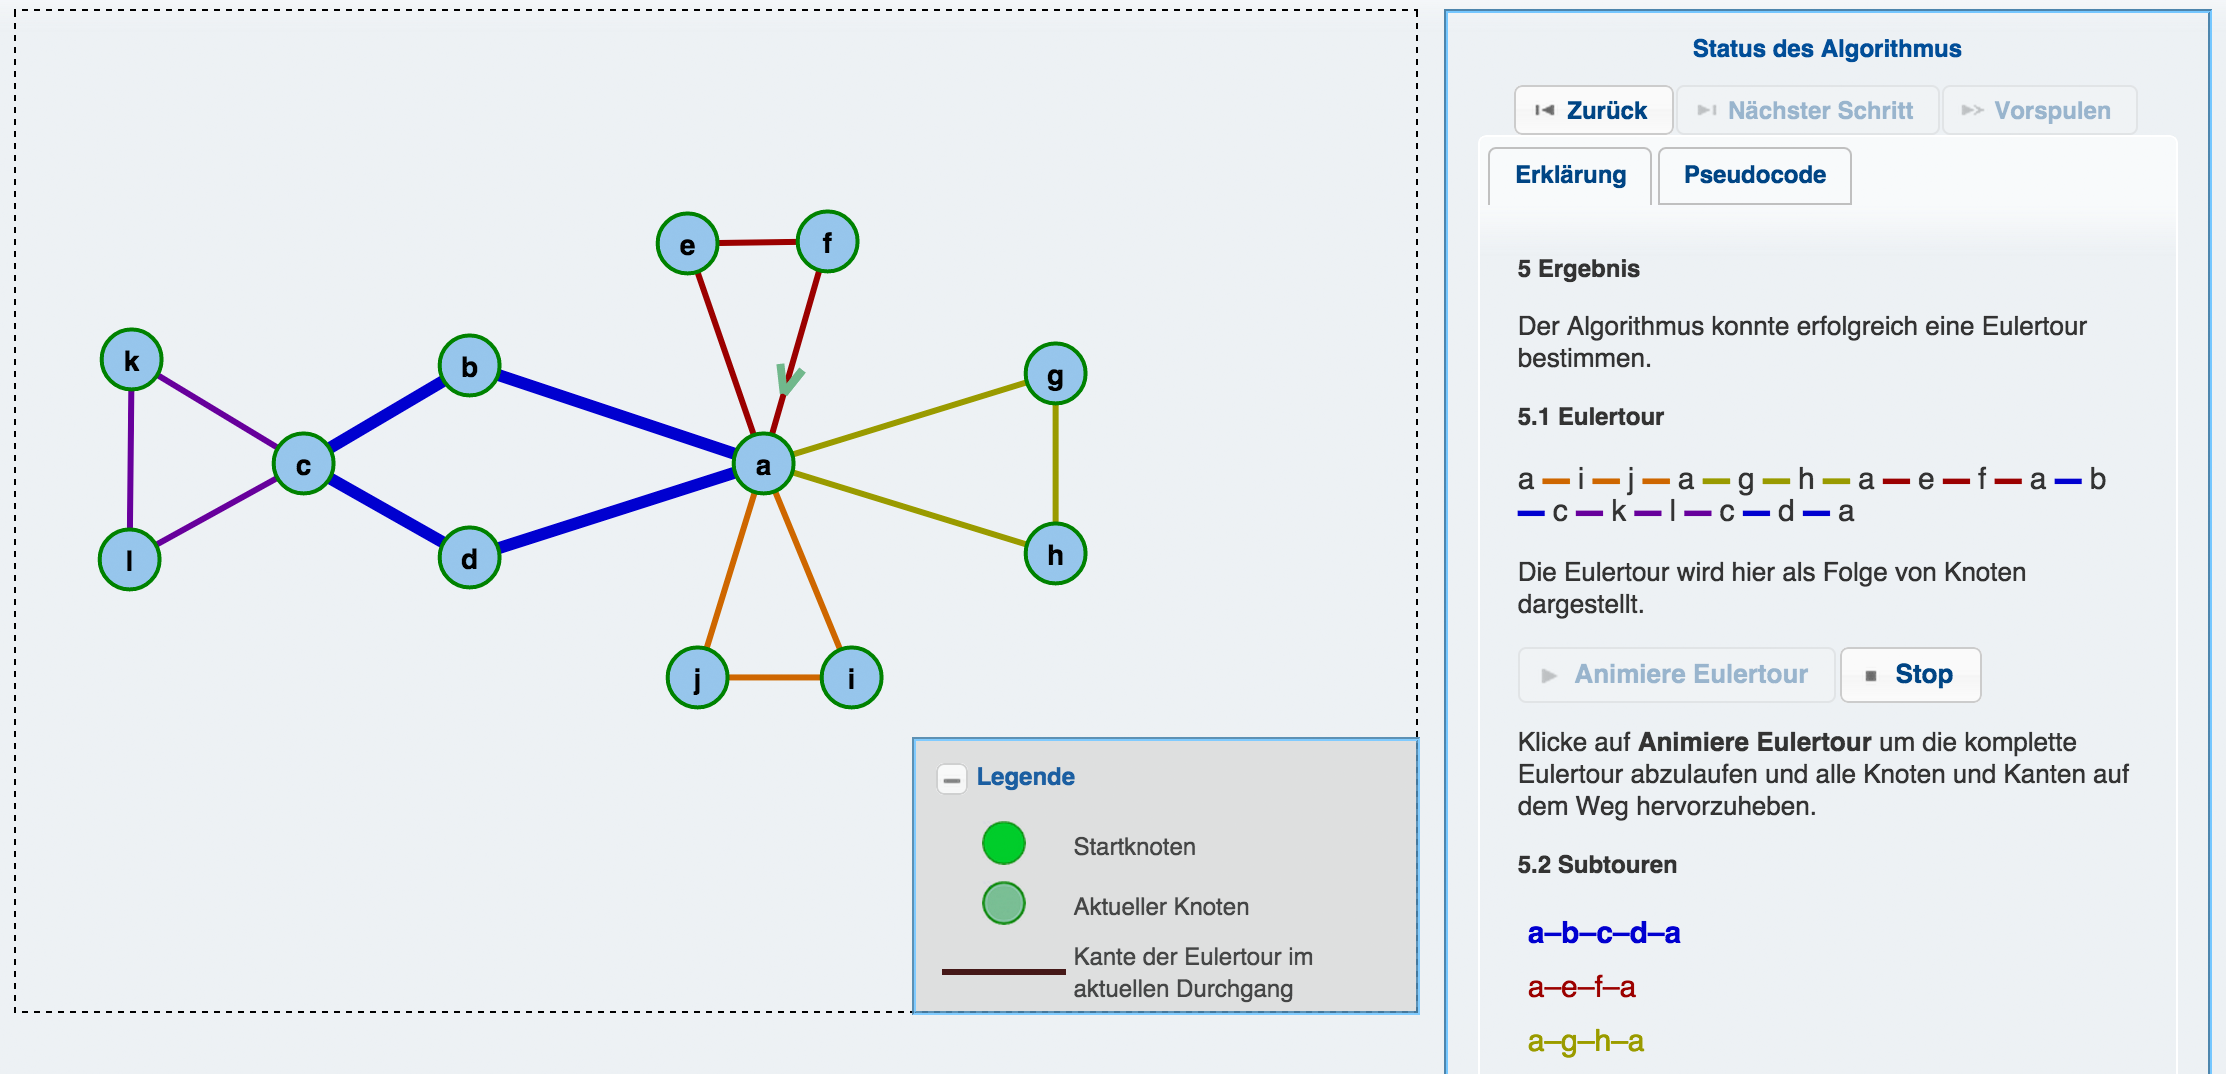
\includegraphics[width=\textwidth]{figures/hierholzer_animation}
	\caption[Eulertour Animation]{Visualisierung der Eulertour mittels Animation}\label{fig:hierholzer-animation}
\end{figure}

Die erste Forschungsaufgabe soll sicherstellen, dass der Nutzer die wichtigsten Abläufe des Algorithmus versteht. Sie behandelt daher im Wesentlichen den Ablauf des Algorithmus, das Konzept des Knotengrads und das Verbinden von Touren.

In einer weiteren Forschungsaufgabe werden die Besonderheiten des Algorithmus bei Anwendung auf einen gerichteten Graphen betrachtet. Der Nutzer betrachtet die geänderten Voraussetzungen, die der Graph erfüllen muss und die veränderte Auswahl der Kanten zur Konstruktion von Subtouren.
     
\section{Algorithmus von Hopcroft und Karp}%Ruslan
Der Algorithmus wurde in Phasen unterteilt. In jeder Phase des Algorithmen wird nach einer inklusions-maximalen Menge von kürzesten disjunkten Augmentationswegen gesucht. Die in einer Phase gefundenen Augmentationswege werden nacheinander hervorgehoben und das Matching augmentiert.
Das Aufzeigen der Augmentationswege stand im Fokus bei der Visualisierung des Algorithmen. Der Benutzter sollte diese leicht erkennen und nachvollziehen können. Um das Konzept von disjunkten Augmentationswegen zu verdeutlichen, werden die Knoten der bereits verarbeiteten Augmentationswegen grau markiert. Dadurch wird dem Benutzer verdeutlicht, dass ein Knoten in einer Phase nur auf einem Augmentationsweg vorkommt. 
Die graue Markierung der benutzten Knoten sollte außerdem hervorheben, dass die Menge von disjunkten Augmentationswegen inklusions-maximal ist. Der Benutzer kann am Ende einer Phase leicht nachvollziehen, dass es keinen weiteren disjunkten kürzesten Augmentationsweg existiert.

\begin{figure}[h!]
	\centering
	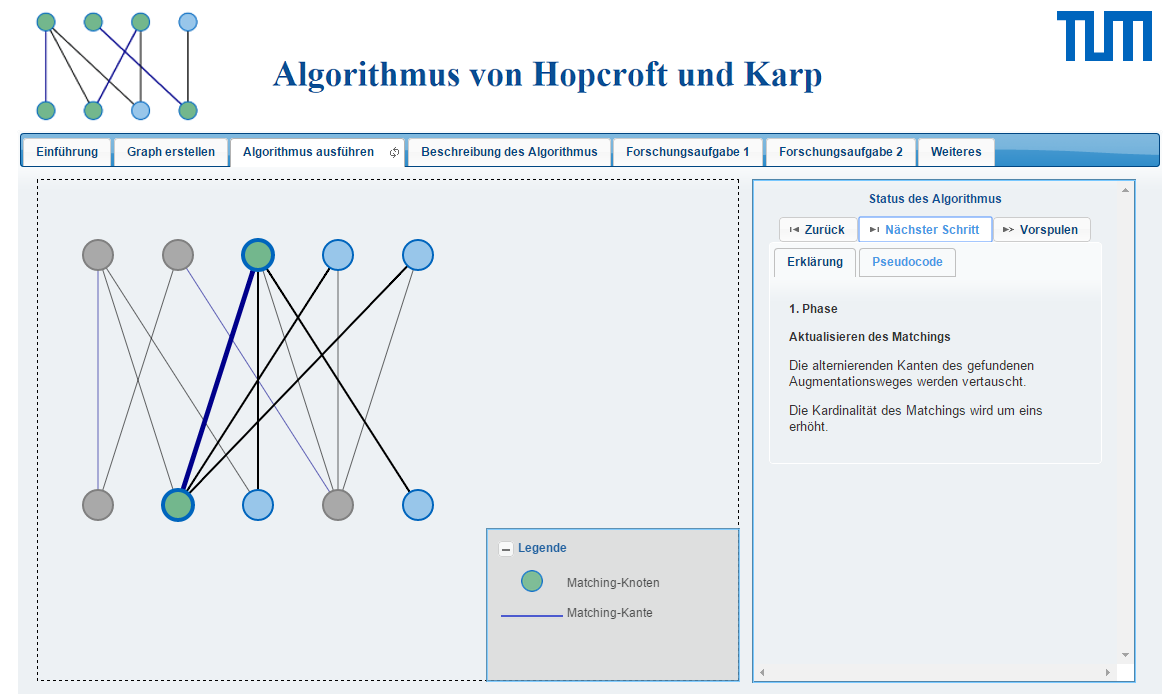
\includegraphics[width=\textwidth]{figures/hopcroft_karp_augmentation}
	\caption[Augmentationsweg]{Hervorhebung des aktuellen Augmentationsweges im Hopcroft-Karp-Algorithmus}\label{fig:hopcroft_karp_augmentation}
\end{figure}

In der ersten Forschungsaufgabe soll der Nutzer sein Verständnis über den Ablauf des Algorithmen prüfen. Der Benutzer sollte das Konzept von kürzesten Augmentationswegen verstehen und wissen, welche Kanten nach einem Augmentationsschritt im Matching sein werden.

In der zweiten Forschungsaufgabe bekommt der Nutzer die Gelegenheit mit Augmentationswegen zu experimentieren. Der Algorithmus stoppt zufällig an einigen Stellen, wo der Benutzer einen Augmentationsweg selbst einzeichnen soll. Es müssen nicht die kürzesten Augmentationswege eingezeichnet werden. Der Benutzer sollte sehen, wie seine Wahl die weitere Ausführung des Algorithmen beeinflusst.

\section{Ungarische Methode}
Besonderheiten Visualisierung
Forschungsfragen

\section{Chinese-Postman-Algorithmus}%Ruslan
%Besonderes
Der implementierte Chinese-Postman-Algorithmus löst das gerichtete Chinese-Postman-Problem. 
Das Besondere bei dem Chinese-Postman-Algorithmus ist, dass er für die Ausführung weitere Algorithmen benötigt. Diese sind 
\begin{itemize}
\item Floyd-Warshall-Algorithmus
\item Ungarische Methode
\item Hierholzer-Algorithmus
\end{itemize}
Der Algorithmus ist in verschiedene Schritte eingeteilt. Zuerst wird überprüft, ob das Problem auf dem Graphen lösbar ist. Anschließend wird eine Menge von Pfaden gesucht, sodass nach dem Einfügen dieser Pfade in den Graphen der Graph eulersch wird. Die Summe der Längen dieser Pfade sollte minimal sein.
Zum Schluss wird ein Eulerkreis im Graphen gefunden, was die Lösung des Problems darstellt.

%Visualisierung
Um die optimale Menge von zusätzlichen Pfaden zu bestimmen, werden zuerst Knoten bestimmt, bei denen die Anzahl der Eingangs- und Ausgangskanten nicht übereinstimmt.
Abhängig davon, ob es zu viele Eingangs- oder Ausgangsknoten gibt, werden diese Knoten hell- bzw. dunkelfarbig markiert(vgl. Abbildung~\ref{fig:unbalanced}). Außerdem wird die Differenz zwischen Ausgangs- und Eingangsgrad eines Knoten im Knoten gezeigt. Dadurch entstehen zwei Partitionen von Knoten. 
%Der Nutzer sieht damit sofort, zwischen welchen Knoten neue Pfade eingefügt werden müssen.

\begin{figure}[h!]
	\centering
	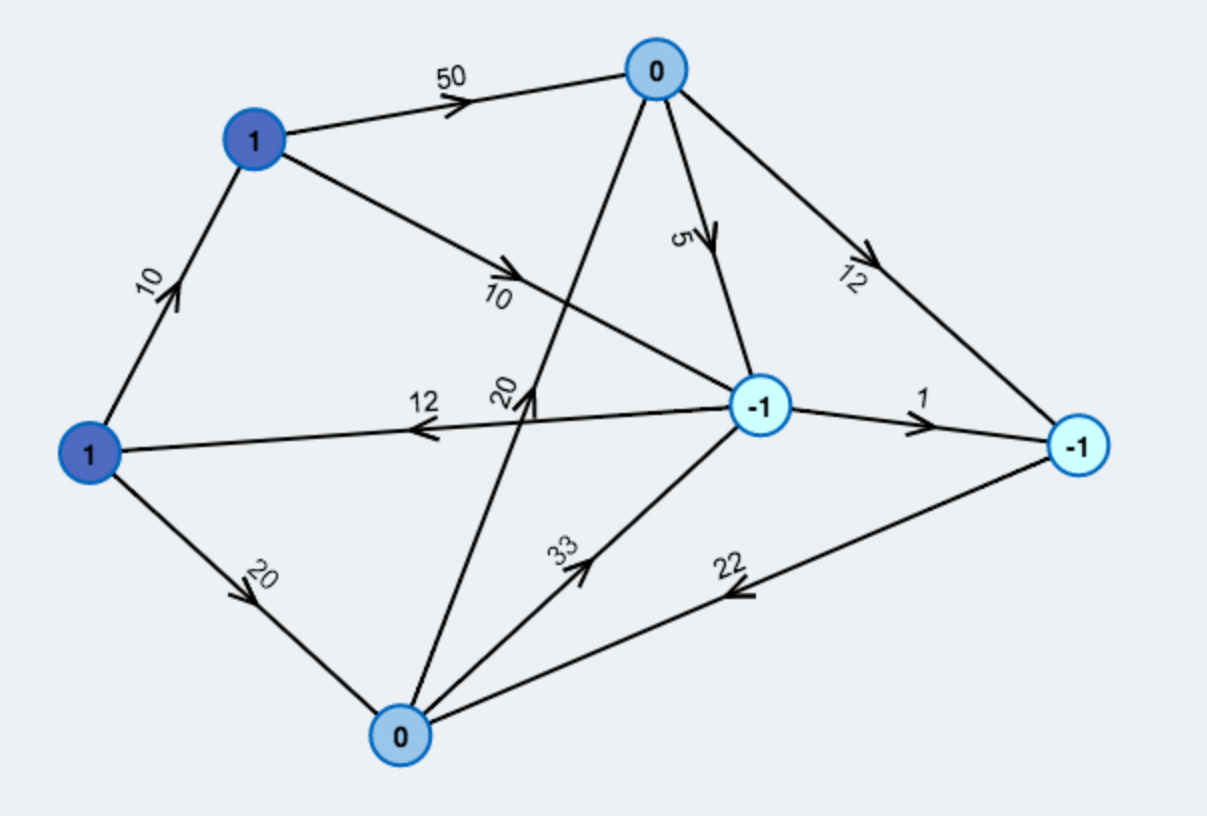
\includegraphics[width=0.8\textwidth]{figures/postman_unbalanced}
	\caption[Unbalancierte Knoten]{Hervorheben von Knoten mit ungleichem Eingangs- und Ausgangsgrad}\label{fig:postman_unbalanced}
\end{figure}

Im nächsten Schritt wird ein bipartiter Graph erstellt, der aus den markierten Knoten besteht. Um den Wechsel von dem Ausgangsgraphen zu dem bipartiten Graphen nachvollziehbar zu gestalten, wurde eine Animation eingefügt. Alle für den Matching-Graphen relevanten Knoten werden aus dem Graphen herausgenommen und zu dem bipartiten Matching-Graphen transportiert. Das Aussehen des Matching-Graphen wurde aus der Ungarischen Methode übernommen. 

\begin{figure}[h!]
	\centering
	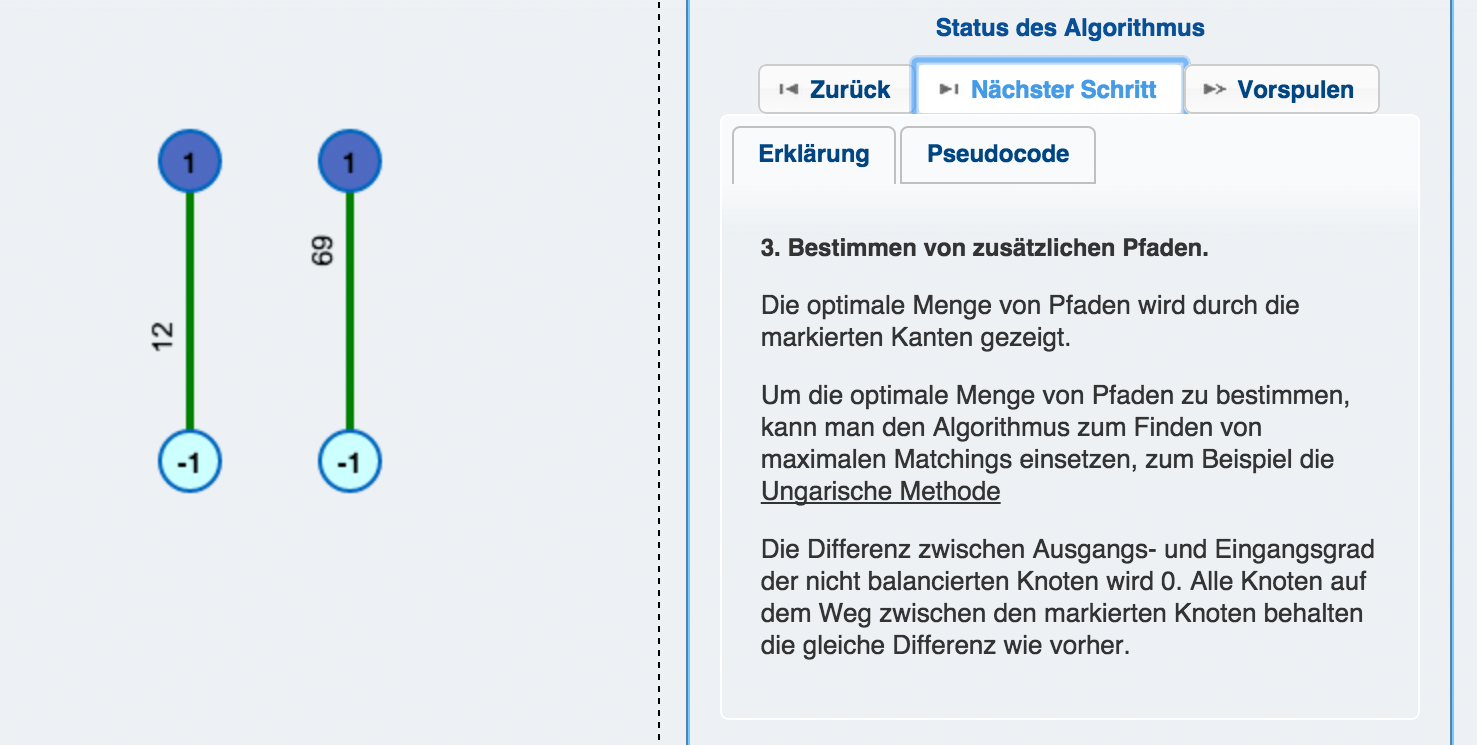
\includegraphics[]{figures/postman_matching}
	\caption[Matching]{Matchinggraph }\label{fig:postman_matching}
\end{figure}

In der Implementierung des Algorithmen bestimmt die Differenz zwischen Ausgangs- und Eingangsgrad eines Knotens, wie oft dieser im Matching-Graphen vorkommt. Es entsteht ein vollständiger bipartiter Graph, sodass mit der Ungarischen-Methode-Algorithmus ein optimales Matching bestimmt werden kann. Das Gewicht einer Kante ist die Länge des kürzesten Weges von dem Knoten mit negativer Differenz zwischen Ausgangs- und Eingangsgrad zu dem Knoten mit positiver Differenz. Bei der Visualisierung des Algorithmen wurde eine Entscheidung zugunsten Übersichtlichkeit getroffen, sodass ein Knoten nur einmal im Matching-Graphen vorkommen sollte. Dadurch wird für den Nutzer nachvollziehbar, zwischen welchen Knoten neue Wege eingefügt werden müssen. Die Differenz zwischen Ausgangs- und Eingangsgrad eines Knotens bestimmt die Anzahl von Pfaden, die in diesem Knoten enden bzw. anfangen müssen und somit die Anzahl von Matching-Kanten, die zu diesem Knoten inzident sind.

Nachdem die optimalen Pfade im Matching-Schritt bestimmt wurden, werden die Knoten wieder an ihren Platz in den normalen Graphen transportiert. Allerdings werden die Matching-Kanten ebenfalls in den Graphen übernommen. Der Benutzer sieht somit auch im normalen Graphen, zwischen welchen Knoten neue Wege eingefügt werden müssen.
Das Einfügen von neuen Pfaden wird ebenfalls mittels einer Animation aufgezeigt. Die aktuelle Matching-Kante wird markiert und die Kanten auf dem neuen Weg werden schrittweise in den Graphen eingefügt. Anschießend wird die Matching-Kante gelöscht.

Am Ende des Algorithmen wird die Eulertour des Graphen bestimmt. Der Nutzer kann die Animation der Tour selbst starten und stoppen. Die Visualisierung der Eulertour ist aus dem Hierholzer-Algorithmus übernommen.

\begin{figure}[h!]
	\centering
	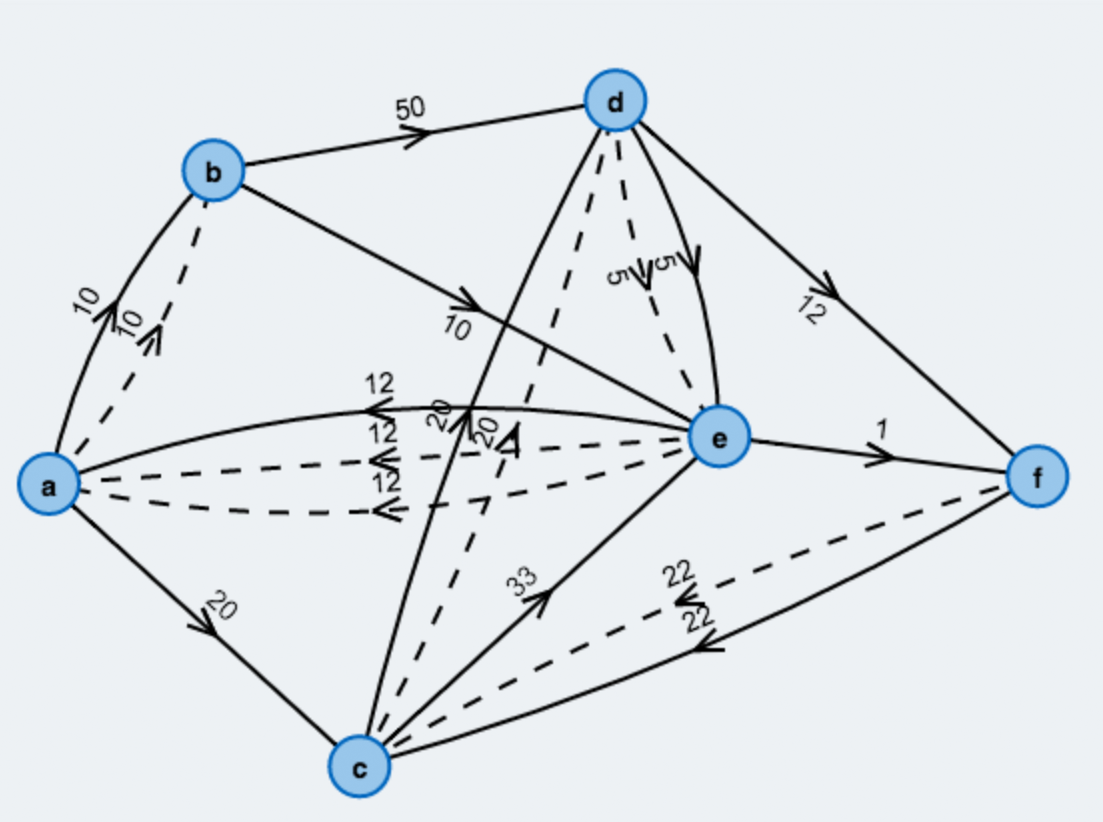
\includegraphics[width=0.8\textwidth]{figures/postman_eulerian}
	\caption[Eulerscher Graph]{Graph nach Einfügen von zusätzlichen Pfaden}\label{fig:postman_eulerian}
\end{figure}

%Forschungsaufgaben
Die erste Forschungsaufgabe sollte das Wissen des Benutzers prüfen. Der Benutzer sollte verstehen, welche Knoten im Matching-Graphen gebraucht werden und wie viele zusätzliche Wege in einem Knoten starten bzw. enden müssen.

Die zweite Forschungsaufgabe lässt dem Benutzer die Möglichkeit den Rundweg selbst zu bestimmen, der alle Kanten des Graphen enthält. Anschließend wird die Länge dieses Weges mit der optimalen Lösung verglichen. Der Benutzer kann dadurch feststellen, inwiefern seine Lösung von der optimalen Lösung abweicht.

\chapter{Implementierung}

\section{Installation (Mark)}
Zur Installation sind keine speziellen Anforderungen zu erfüllen. Die Webapplikationen wurden vollständig mittels HTML5, JavaScript und CSS implementiert, sodass keine zusätzliche serverseitige Software benötigt wird. Zum Aufrufen der Anwendungen wird ein moderner Webbrowser benötigt.

Die Bereitstellung erfolgt über den Online Dienst GitHub, der das verteile Versionskontrollsystem Git benutzt. 
Alle Anwendungen liegen in einem gemeinsamen Repository, welches unter \url{https://github.com/herzog31/adv-graph-algorithms} erreichbar ist. Zur Installation kann man entweder auf der Repository Seite die letzte freigegebene Version (Release) als Zip oder Tar Archiv herunterladen oder die aktuellste Version des Repositories mittels folgendem Befehl in das aktuelle Verzeichnis kopieren.

\begin{figure}[h!]
\begin{lstlisting}[language=Bash]
git clone -b master https://github.com/herzog31/adv-graph-algorithms.git
\end{lstlisting}
\caption[Repository Kopieren]{Befehl zum Kopieren des GitHub Repositories}\label{fig:listing-github}
\end{figure}

Um die Anwendungen als Webanwendungen online bereitzustellen wird ein Webserver benötigt. Hier emfiehlt sich die Installation des Apache oder nginx  HTTP Servers.

Die lokale Ausführung ist ohne einen Webserver möglich. Verschiedene Webbrowser besitzen allerdings eine Sicherheitsrichtlinie, die das Öffnen von lokalen Dateien über JavaScript verbieten. Diese Sicherheitsrichtline kann jedoch durch spezielle Einstellungen umgangen werden. Für Google Chrome ist dies über den Start Parameter \texttt{--allow-file-access-from-files} möglich.

\section{MathJAX (Mark)}
Unter den Tabs \enquote{Beschreibung des Algorithmus} werden die komplizierten Algorithmen, wie bspw. die Ungarische Methode, in möglichst einfachen Worten als Fließtext erklärt. Wir gehen davon aus, dass der Nutzer während der Bearbeitung der Forschungsaufgaben, verschiedene Sachverhalte in der Algorithmenbeschreibung nachschlagen muss. Das wiederholte Lesen von vollständigen Absätzen wollten wir allerdings vermeiden.

Dazu haben wir zusätzlich zur textuellen Beschreibung, wichtige Punkte der Algorithmen auch als mathematische Formeln dargestellt. Der Nutzer erlangt so durch das erste Lesen der Beschreibung ein Grundverständnis der Algorithmen und kann während der Bearbeitung aufkommende Fragen durch die dargestellten Formeln schneller erschließen.

Zur Darstellung der Formeln in den Webapplikationen verwenden wir JavaScript Bibliothek MathJAX\footnote{https://www.mathjax.org/}. Diese ist frei unter der Apache-Lizenz erhältlich und wird u.a. auch von Wikipedia zur Darstellung jeglicher mathematischer Ausdrücke genutzt. Mit der Bibliothek ist es möglich mit LaTeX beschriebene Ausdrücke als SVG oder PNG im Webbrowser zu rendern. 

Damit die Bibliothek in den Webanwendungen genutzt werden kann, muss sie wie folgt eingebunden werden (vgl. Abbildung~\ref{fig:listing-mathjax-include}.

\begin{figure}[h!]
\begin{lstlisting}[language=HTML]
<script type="text/javascript" src="../library/js/mathjax/MathJax.js?config=TeX-AMS-MML_SVG.js&locale=de"></script>
<script type="text/x-mathjax-config">
	MathJax.Hub.Config({
		showMathMenu: false,
		showMathMenuMSIE: false
	});
</script>
\end{lstlisting}
\caption[MathJAX Einbindung]{Einbinden der MathJAX Bibliothek}\label{fig:listing-mathjax-include}
\end{figure}

Nach der Einbindung werden sämtliche LaTeX Ausdrücke welche sich zwischen den Begrenzungszeichen \texttt{\textbackslash(} und \texttt{\textbackslash)} befinden, automatisch übersetzt. In einem Beispiel wird hier der HTML Code in Abbildung~\ref{fig:listing-mathjax-example-html} von MathJAX im Browser gerendert (vgl. Abbildung~\ref{fig:mathjax-example-img}.

\begin{figure}[h!]
\begin{lstlisting}[language=HTML]
<p style="text-align: center;">
	\(\Delta = \min\limits_{s \in S\ \wedge\ y \in Y \setminus T}\{l(s) + l(y) - w(s,y)\}\)
</p>
\end{lstlisting}
\caption[MathJAX Beispiel Code]{MathJAX Beispiel: HTML Code}\label{fig:listing-mathjax-example-html}
\end{figure}

\begin{figure}[h!]
	\centering
	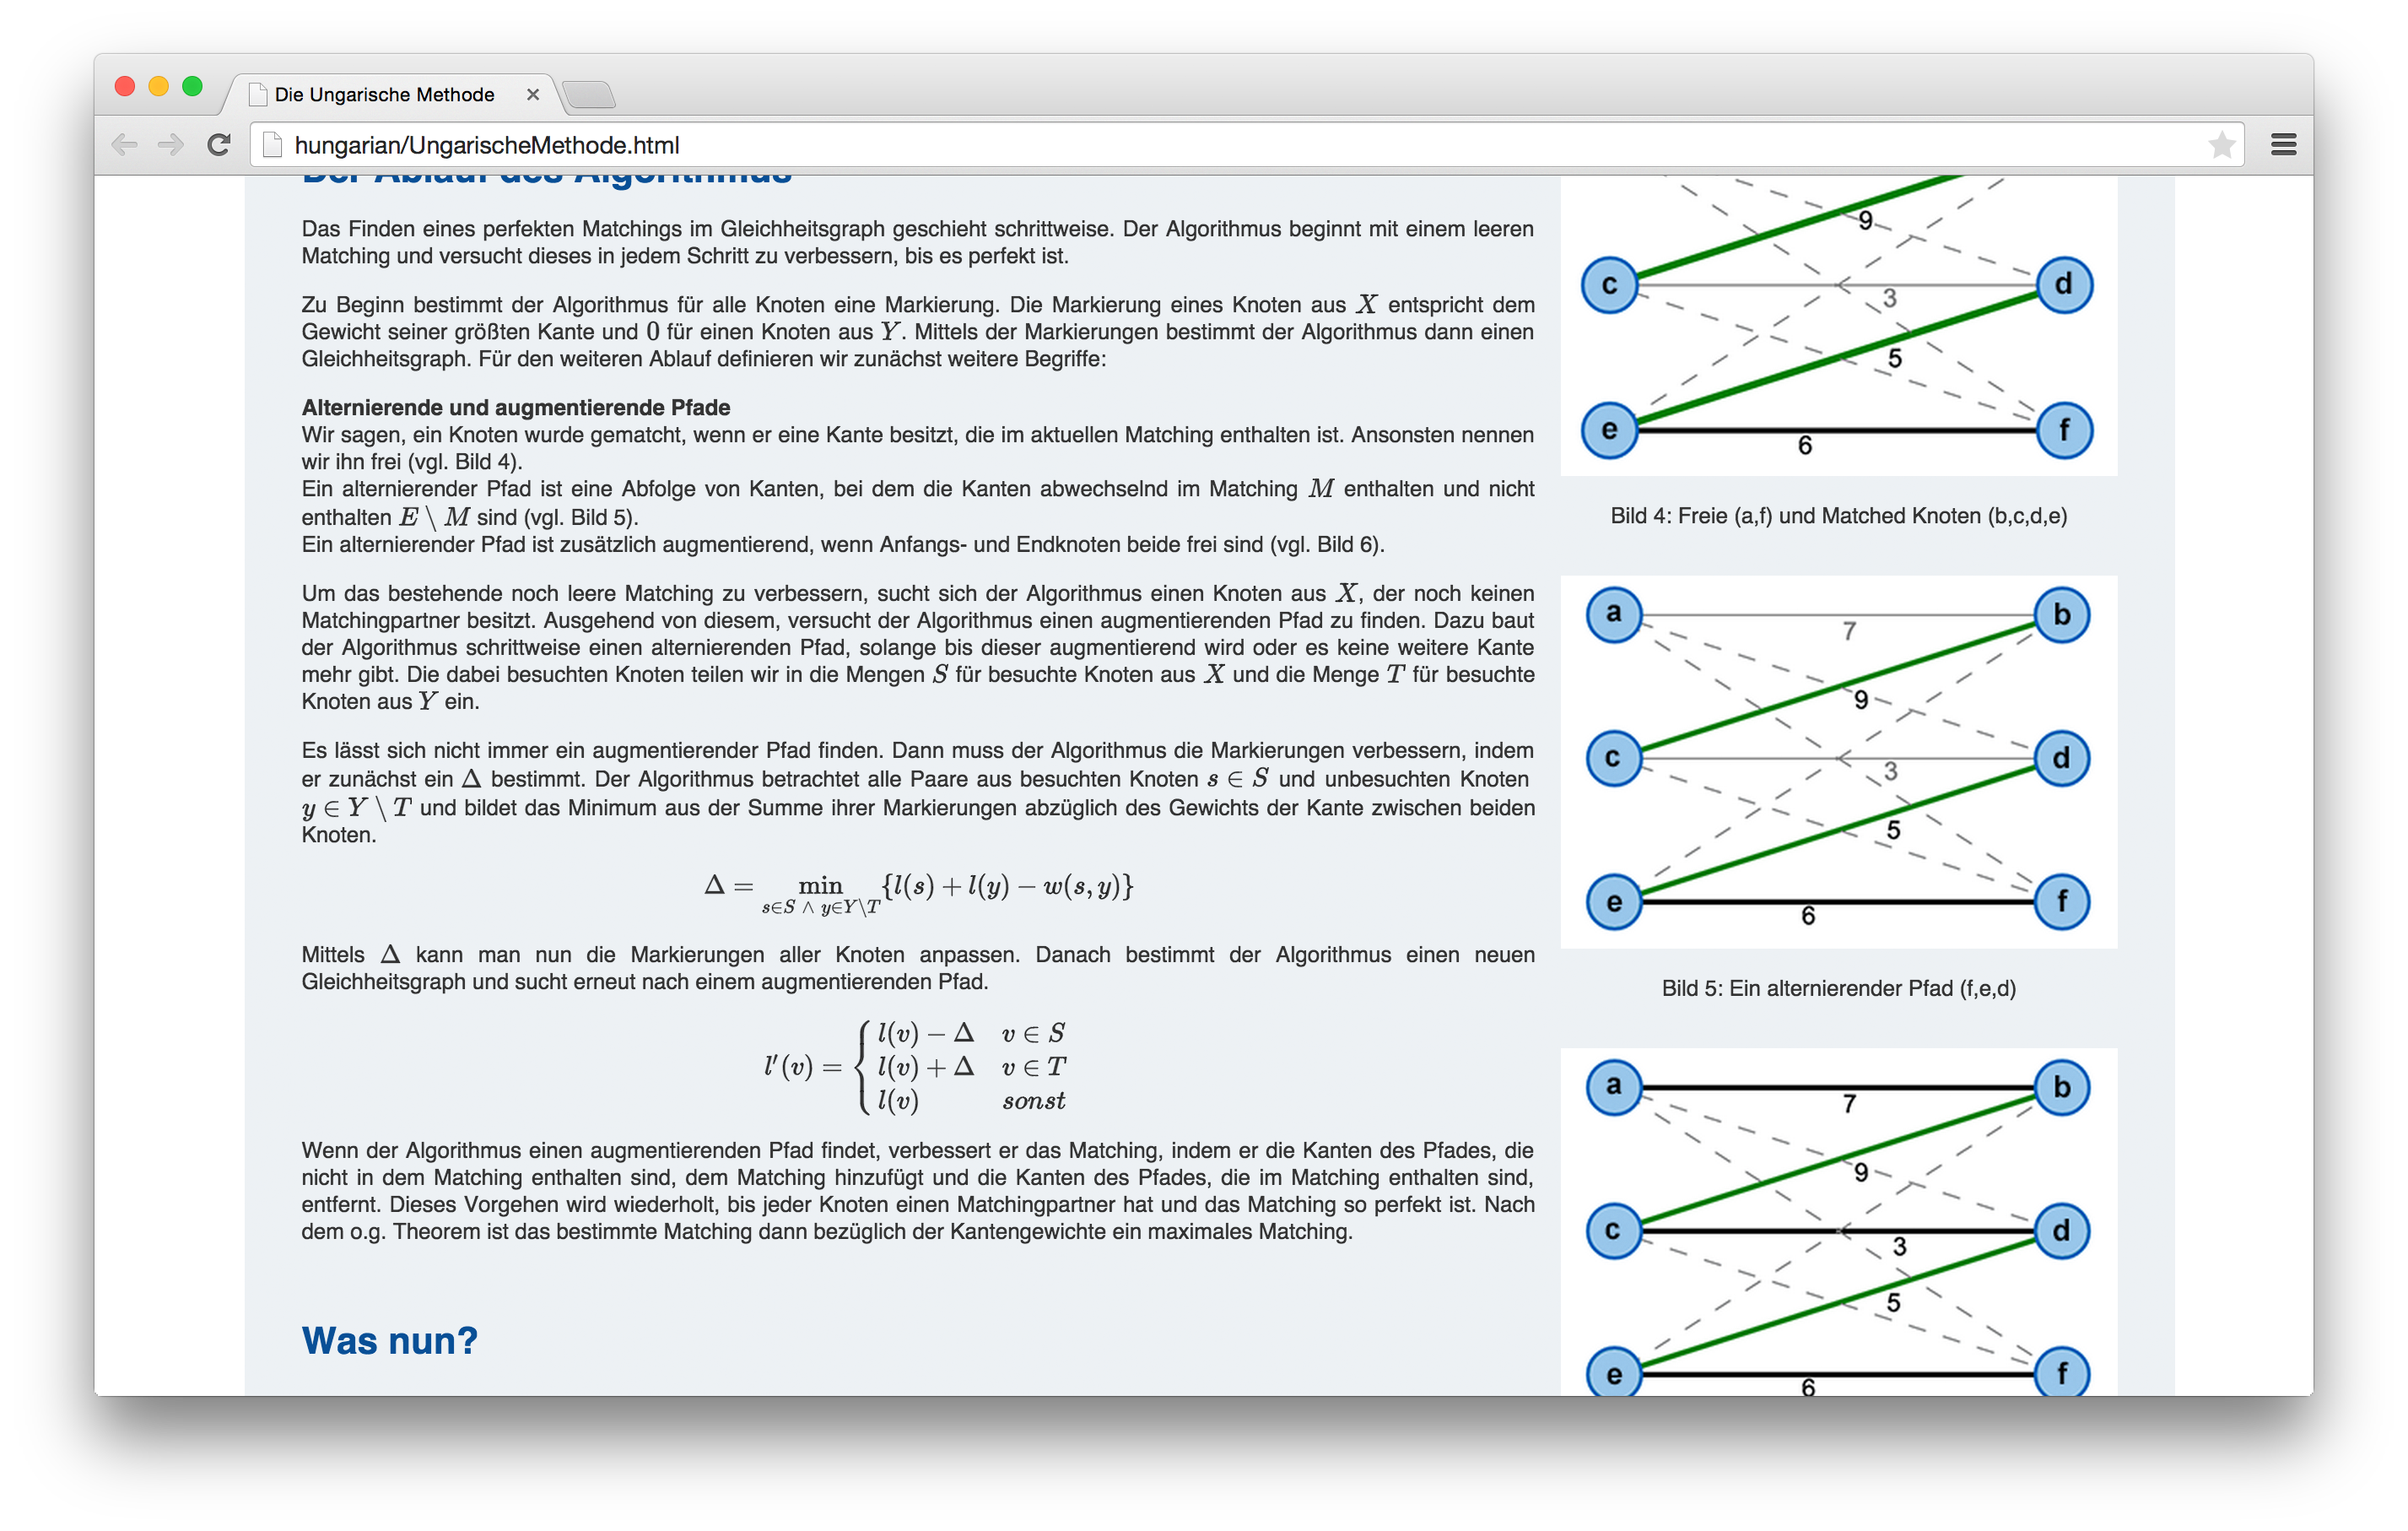
\includegraphics[width=\textwidth]{figures/mathjax-example}
	\caption[MathJAX Beispiel Browser]{MathJAX Beispiel: Darstellung im Browser}\label{fig:mathjax-example-img}
\end{figure}

Werden Ausdrücke zur Laufzeit in das DOM mittels JavaScript eingefügt, so müssen diese separat übersetzt werden (vgl. Abbildung~\ref{fig:listing-mathjax-render}).

\begin{figure}[h!]
\begin{lstlisting}[language=JavaScript]
MathJax.Hub.Queue(["Typeset", MathJax.Hub]);
\end{lstlisting}
\caption[MathJAX Render Befehl]{Befehl zum erneuten Rendern von Ausdrücken im HTML Dokument}\label{fig:listing-mathjax-render}
\end{figure}

\section{Bipartite Graphen}
Motivation
Beispiel

\section{Multigraphen}%Ruslan
%Motivation
In bisherigen auf dem Framework basierenden Algorithmen war es nicht möglich Multikanten zu erstellen, was aber für die Algorithmen nicht notwendig war. Es war möglich maximal zwei Kanten zwischen zwei Knoten einzufügen. 
In dem Chinese-Postman-Algorithmus werden während der Ausführung Kanten in den Graphen eingefügt. Deshalb muss das Graphenmodell für den Chinese-Postman-Algorithmus mit Multikanten darstellen können. Die Abbildung \ref{fig:multigraph} zeigt einen Graphen mit Multikanten.
%Beispiel
\begin{figure}[h!]
	\centering
	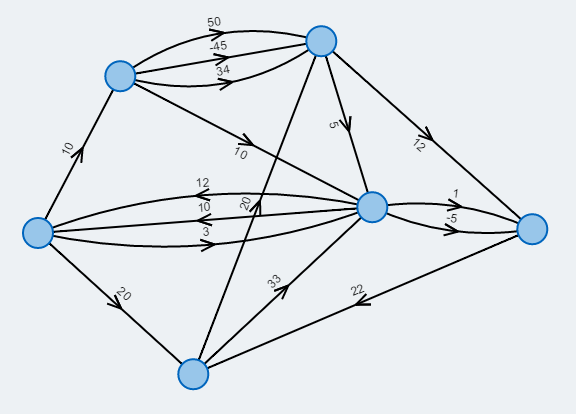
\includegraphics[width=\textwidth]{figures/multigraph}
	\caption[Multigraph]{Multikanten im Graphen}\label{fig:multigraph}
\end{figure}

\section{Zufällig generierte Fragen (Mark)}
In bisherigen auf diesem Framework basierenden Projekten war die Varianz der Fragen in den Forschungsaufgaben problematisch. Die Forschungsaufgaben behandelten meistens statische Fragen an vorher festgelegten Stellen zu vorgegebenen Graphen. Daraus resultierend bietet sich dem Nutzer ein wenig abwechslungsreiches Erlebnis und die Motivation, eine Forschungsaufgabe mehrfach zu bearbeiten, ist nicht gegeben.

In unserer Implementierung verfolgen wir daher einen anderen Ansatz. Die Forschungsaufgaben sind grundsätzlich so aufgebaut, dass sie die gleiche Struktur und den gleichen Quellcode wie die reguläre Ausführung des Algorithmus benutzen. Das schließt auch den vom Nutzer selbst gewählten Graph aus dem \enquote{Graph erstellen} Tab mit ein. Statt statischen Fragen definiert der Entwickler eine Menge von Fragetypen. Vor jedem Schritt des Algorithmus wird dann anhand einer Wahrscheinlichkeitsmatrix bestimmt, ob zu dem folgenden Schritt eine Frage gestellt wird und wenn ja, welcher Fragetyp gewählt werden soll. Außerdem sollen wenn möglich die Inhalte der generierten Fragen eines Fragetyps variieren. So werden beispielsweise die Knoten, zu denen ein Wert bestimmt werden soll, zufällig gewählt (vgl. Abbildung~\ref{fig:random-question}).

Mit dieser Implementierung gelingt es, dass in jeder Bearbeitung einer Forschungsaufgabe unterschiedliche Kombinationen von Fragen gestellt werden. Zusätzlich kann der Nutzer durch selbst erstelle Graphen auch Spezialfälle testen.

\begin{figure}[h!]
	\centering
	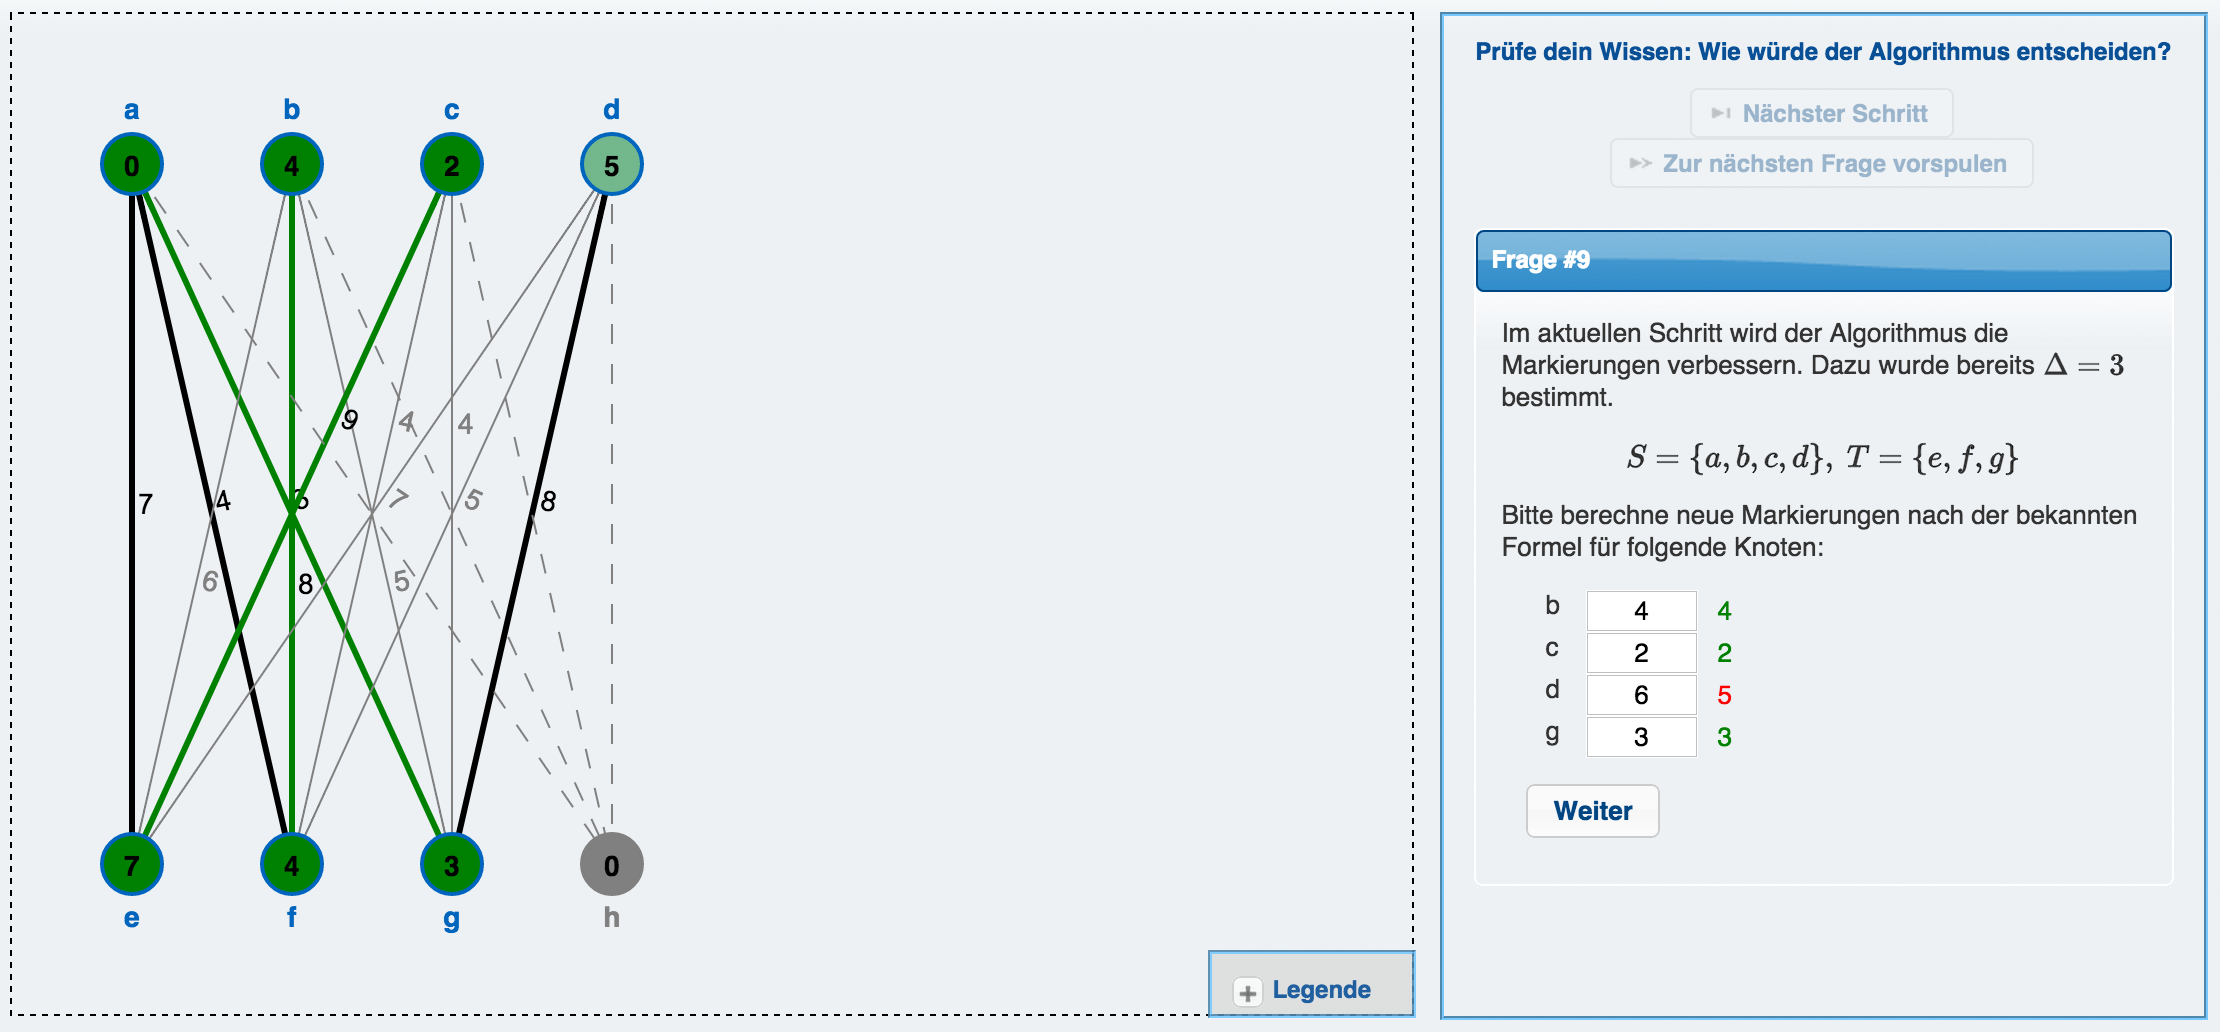
\includegraphics[width=\textwidth]{figures/random_question}
	\caption[Zufällig generierte Frage]{Beispiel für eine zufällig generierte Frage}\label{fig:random-question}
\end{figure}

\subsection*{Implementierung}
In der Funktion \texttt{this.nextStepChoice} wird vor der Auswahl des nächsten Schritts des Algorithmus mittels der Funktion \texttt{this.askQuestion} bestimmt, ob und welche Frage gestellt werden soll. Für jeden Fragetyp exisiert eine separate Funktion (bspw. \texttt{this.generateNextStepQuestion}), die auf den aktuellen Graph zugreift und eine Frage mit zufälligen Elementen generiert und in das DOM Element \texttt{\#tf1\_div\_questionModal} schreibt. Die gegebene Antwort wird durch Aufruf der Funktion \texttt{this.saveAnswer} gespeichert und mit der richtigen Lösung verglichen. Am Ende der Forschungsaufgabe kann mittels \texttt{this.showQuestionResults} eine Übersicht angezeigt werden, die zeigt, wieviele Fragen richtig beantwortet wurden. Weitere Informationen sind der Inline-Dokumentation zu entnehmen.

\section{Gemeinsam genutzte Dateien (Mark)}
Im Rahmen dieses interdisziplinären Projekts wurden Webapplikationen für insgesamt fünf Algorithmen entwickelt. Jede Applikation liegt in einem von den anderen Algorithmen unabhängigen Projektordner, der jeweils auch das Graph Framework aus früheren Projekten enthält. Daher lagen im gesamten Repository viele Dateien mehrfach vor. Dies war insofern problematisch, da Änderungen, die alle Anwendungen betreffen in mehreren Dateien vorgenommen werden mussten.

Unser Ziel war es daher, gemeinsam genutzte Dateien auszulagern. Wir beschränken uns hier auf Dateien, welche das Layout und Design der Anwendungen definieren sowie universelle Programmbibliotheken (bspw. MathJAX). Diese Beschränkung ist notwendig, um die Flexibilität im Entwicklungsprozess zu gewährleisten. Es existieren weitere Dateien, die sich zum aktuellen Zeitpunkt anwendungsübergreifend nicht signifikant unterscheiden. Diese sind allerdings algorithmenspezifisch und könnten in zukünftigen Entwicklungsphasen weiter verändert werden.

Zur Auslagerung legten wir zunächst einen \texttt{library} Ordner an. Das Finden von Dateiduplikaten übernimmt ein Python Skript (vgl. \texttt{deduplicate.py}), welches mittels der \texttt{difflib} Bibliothek alle Dateien in den Projektordnern paarweise miteinander vergleicht und einen Ähnlichkeitsquotienten bestimmt. Das Skript zeigt dann alle Dateien, die einen festgelegten Änhlichkeitsgrenzwert überschreiten an (vgl. Abbildungen \ref{fig:shared-files-1} und \ref{fig:shared-files-2}). Anhand des Quotienten lässt sich ablesen, ob Dateien im Gesamten oder in Teilen ausgelagert werden können. Das Verschieben in den \texttt{library} Ordner und die Anpassung der Pfade in den Anwendungen erfolgt dann manuell.

\begin{figure}[h!]
\noindent\texttt{chinese-postman/img/TUMLogo.png \\
-> 100.00\% identical to floyd-warshall/img/TUMLogo.png \\
-> 100.00\% identical to hierholzer/img/TUMLogo.png \\
-> 100.00\% identical to hopcroft-karp/img/TUMLogo.png \\
-> 100.00\% identical to hungarian/img/TUMLogo.png
}
\caption[Gemeinsame Dateien, Beispiel 1]{Vollständige Übereinstimmung bei der Datei \texttt{TUMLogo.png}}\label{fig:shared-files-1}
\end{figure}

\begin{figure}[h!]
\noindent\texttt{chinese-postman/js/siteAnimation.js \\
-> 67.01\% identical to hierholzer/js/siteAnimation.js \\
-> 91.49\% identical to hopcroft-karp/js/siteAnimation.js \\
-> 71.13\% identical to hungarian/js/siteAnimation.js
}
\caption[Gemeinsame Dateien, Beispiel 2]{Mäßige Übereinstimmungen bei der Datei \texttt{siteAnimation.js}}\label{fig:shared-files-2}
\end{figure}

Für zukünftige Projekte können die Parameter des Skripts angepasst werden. Weitere Informationen hierzu sind der Inline-Dokumentation zu entnehmen.

\chapter{Zusammenfassung}
Zusammenfassung der wesentlichen Punkte
%% conclusion.tex
%%

%% ==================
\chapter{Zum Weiterlesen}
\label{ch:reader}
%% ==================

In diesem Kapitel sammeln wir ein paar Literaturhinweise in Sachen \LaTeX, die
Anfängern und Fortgeschrittenen Anwendern den Einstieg erleichtern und
vielleicht einige nützliche Hinweise geben können.
\begin{description}
\item[lshort:] \enquote{The Not So Short Introduction to \LaTeX}
  (vgl. \cite{l2short}) ist eine aktuelle Einführung, die sich mit moderatem
  Zeitaufwand zum Einstieg durcharbeiten lässt (die Autoren geben für die zum
  Zeitpunkt der Erstellung dieses Dokuments aktuelle Version 5.01 eine Zeit von
  157 Minuten an). Die jeweils aktuelle Version findet man auf
  \url{http://tobi.oetiker.ch/lshort/lshort.pdf}.
\item[\LaTeX{} and Friends:] Das Buch \cite{vanDongen2012} ist eine
  empfehlenswerte und aktuelle Einführung in  \LaTeX, die viele aktuelle Pakete
  behandelt. Für Einsteiger wie auch für Fortgeschrittene einen Blick wert.
\item[l2tabu:] In \cite{l2tabu} sind einige Hinweise auf veraltete Pakete und
  \LaTeX-Befehle enthalten, die besonders für Fortgeschrittene \LaTeX-Nutzer
  lesenswert sind. Hier erfährt man, warum man bestimmte Kommandos besser nicht
  einsetzen sollte und was bessere Alternativen sind. Übrigens: Die Klasse
  \texttt{tumthesis.cls} bindet automatisch das Paket \texttt{nag} ein, das bei
  vielen in l2tabu gelisteten Fehler direkt Alarm schlägt.
\end{description}

%%% Local Variables: 
%%% mode: latex
%%% TeX-master: "thesis"
%%% End: 



% Eventuelle Anhänge
\appendix
%% appendix.tex
%%

%% ==============================
%\chapter{Appendix}
%\label{ch:Appendix}
%% ==============================

\chapter{Bemerkungen zur Implementierung}
\label{Anhang-Implementierung}
		
Im Anhang können beispielsweise Code-Listings oder weiterführende Bemerkungen
ausgeführt werden, die im Hauptteil den Lesefluss stören würden. Wenn Sie keinen
Anhang benötigen, können Sie diese Datei natürlich auch einfach weglassen (und
dann auch den \verb|\include|-Befehl in \texttt{thesis.tex} löschen).

%%% Local Variables: 
%%% mode: latex
%%% TeX-master: "thesis"
%%% End: 

% Alle Anhänge hinter backmatter werden nicht nummeriert
\backmatter


%Abbildungsverzeichnis
\listoffigures

\vspace*{1.5cm}

Alle Abbildungen in diesem Dokument stammen vom Autor selbst. Zur Erzeugung
wurde das großartige \TeX-Paket TikZ von Till Tantau verwendet, vgl.
\cite{Tantau2007}.

%Tabellenverzeichnis
\listoftables

%Algorithmenverzeichnis
% nur in Verbindung mit algorithm2e
%\phantomsection% fuer hyperref
%\addcontentsline{toc}{chapter}{Algorithmenverzeichnis}%
%\markboth{Algorithmenverzeichnis}{Algorithmenverzeichnis}
%\listofalgorithms

% Index
% Für Index zum Inhaltsverzeichnis hinzu 	
\addcontentsline{toc}{chapter}{Index}
\printindex

% Literaturverzeichnis
\printbibliography[heading=bibintoc]

% In der Endversion sollte das hier leer sein und muss dann nicht auskommentiert
% werden. Wer schlampig arbeitet, sollte aber zumindest daran denken, die
% fixme-Liste hier auszukommentieren, damit die "Baustellen" für die
% KorrektorInnen nicht ganz so offensichtlich sind.
\listoffixmes
%
\end{document}
% ==============================================================================
% Ende des Dokuments
% ==============================================================================